\documentclass[journal]{IEEEtran}

\usepackage[T1]{fontenc}
\usepackage[utf8]{inputenc}
\usepackage{amsmath,amssymb,amsfonts}
\usepackage{booktabs}
\usepackage{multirow}
\usepackage{graphicx}
\usepackage{tikz}
\usetikzlibrary{shapes.geometric, arrows.meta, positioning, calc, fit, backgrounds}
\usepackage{url}
\usepackage{hyperref}
\usepackage{array}
\usepackage{enumitem}
\usepackage{balance}
\usepackage{xcolor}
\usepackage{algorithm}
\usepackage{algpseudocode}

% ─────────────────────────────────────────────────────────────────────────────
\title{Sanshodhak: Adaptive Hybrid Retrieval-Augmented Generation\\
       with Vocabulary-Jaccard Knowledge Graph Expansion\\
       for Scholarly Research Intelligence}

\author{Anonymous Authors%
\thanks{Manuscript submitted February 2026.}}

\markboth{IEEE Transactions on Knowledge and Data Engineering, 2026}%
         {Sanshodhak: AHR-RAG for Scholarly Research Intelligence}

% ─────────────────────────────────────────────────────────────────────────────
\begin{document}
\maketitle

% ─────────────────────────────────────────────────────────────────────────────
\begin{abstract}
Scholarly research assistance demands systems that unify multi-source
literature discovery, robust document ingestion, semantically precise
retrieval, grounded answer generation, and implementation-resource
recommendation—while operating within open-access legal and latency
constraints. We present \textbf{Sanshodhak}, a production-oriented
research-intelligence platform whose central contribution is
\emph{Adaptive Hybrid Retrieval} (AHR): a unified pipeline that fuses
BM25 sparse retrieval, BGE-M3 dense FAISS retrieval, and
vocabulary-Jaccard knowledge-graph expansion through Reciprocal Rank
Fusion (RRF), with a slot-reservation mechanism that guarantees
graph-expanded context even when dense retrieval saturates top-$k$.
Beyond the core AHR pipeline, we contribute four complementary
algorithmic innovations: (i)~\emph{Confidence-Weighted RRF}
(CW-RRF), which replaces uniform list weights with entropy-derived
confidence scores; (ii)~\emph{Adaptive Graph Budget Allocation},
which dynamically sizes the graph-expansion slot count per query
based on retriever uncertainty and out-of-vocabulary ratio;
(iii)~\emph{MMR Diversity Regularisation}, which applies Maximal
Marginal Relevance re-ranking to reduce redundant chunks in the
context window; and (iv)~a \emph{Query Difficulty Classifier} that
routes queries to dense-heavy or graph-heavy retrieval
configurations.
Sanshodhak ingests papers from nine heterogeneous scholarly APIs
(OpenAlex, CORE, Semantic Scholar, ArcSieve, DOAJ, PubMed, CrossRef,
Unpaywall, arXiv), constructs a dual-edge knowledge graph from TF-IDF
vocabulary similarity and bibliographic citation co-occurrence without
external NER tools or graph databases, and ranks candidates with a
composite temporal-aware score weighting citation impact, recency
decay, and open-access accessibility. We conduct a four-way ablation
study comparing Dense Vector Retrieval (VR-D), Hybrid BM25+Dense
(VR-H), Graph-only (GR), and full Adaptive Hybrid Retrieval
(HGR) across 100 standardised retrieval questions and generate answers
via DeepSeek-R1:7b. HGR achieves
P@1\,=\,0.45, NDCG@5\,=\,0.665, NDCG@10\,=\,0.694, MRR\,=\,0.627,
and MAP\,=\,0.609---outperforming the dense baseline by +28.6\% in
Precision@1, +10.0\% in NDCG@5, and +14.8\% in MRR, at a mean
retrieval latency of 152\,ms (CPU-only). Generation quality
reaches ROUGE-1\,=\,0.346 and BERTScore-F1\,=\,0.875. These results provide the first
published four-way ablation contrasting dense, hybrid,
graph-only, and hybrid+graph retrieval on a scholarly corpus with
standardised IR metrics and latency measurement.
\end{abstract}

\begin{IEEEkeywords}
Retrieval-Augmented Generation, Knowledge Graph, Hybrid Retrieval,
Reciprocal Rank Fusion, Scholarly Search, FAISS, BM25, BGE-M3,
Research Intelligence, Information Retrieval
\end{IEEEkeywords}

% ─────────────────────────────────────────────────────────────────────────────
\section{Introduction}
\label{sec:intro}

The modern scholarly research workflow is bottlenecked by
tool fragmentation: one system discovers papers, another downloads
PDFs, a third parses full text, and a fourth supports question
answering. Retrieval-Augmented Generation (RAG) \cite{lewis2020rag}
addresses part of this challenge by grounding neural generation in
retrieved evidence, yet most deployed RAG systems for academic use
rely exclusively on dense vector retrieval~\cite{johnson2019faiss},
leaving substantial performance gains from hybrid and graph-augmented
approaches unrealised.

Modern researchers spend a significant portion of their time—often upwards of 10-15 hours per week—on literature discovery, curation, and synthesis \cite{tenopir2015scholarly}. To address this, Sanshodhak is designed for a specific deployment scenario: open-access, CPU-only, institutional or individual use where reproducibility and privacy are paramount.

Three specific limitations in current RAG architectures motivate this work. First, \emph{dense retrieval under-serves sparse queries}: RAG queries over scientific corpora frequently contain rare abbreviations, acronyms, and methodology names where BM25 \cite{robertson2009probabilistic} consistently outperforms dense models. Second, \emph{knowledge graph construction is often outsourced to external NER pipelines or graph-database infrastructure} (e.g., Neo4j, GraphRAG API), raising deployment costs and data-privacy risks. Third, \emph{multi-source ingestion is typically limited to one or two APIs}, missing coverage from biomedical, open-access directory, and aggregator sources that are critical for interdisciplinary research.

Table~\ref{tab:comparison} contrasts Sanshodhak with standard dense retrieval and existing Knowledge-Graph RAG systems.

\begin{table}[htbp]
\centering
\caption{Comparison of Sanshodhak with Prior RAG Approaches}
\label{tab:comparison}
\begin{tabular}{@{}lccc@{}}
\toprule
\textbf{Feature} & \textbf{Standard RAG} & \textbf{GraphRAG} & \textbf{Sanshodhak (Ours)} \\ \midrule
Retrieval Style & Dense & Graph & Hybrid + Graph (AHR) \\
KG Construction & None & LLM NER Prompting & TF-IDF Vocabulary \\
Graph Database & N/A & Neo4j / External & In-Memory (NetworkX) \\
Ingestion Sources & Single DB & Single DB & 9 Parallel APIs \\
Deployment Scope & Cloud/API & High-Compute & CPU-Only, Local \\ \bottomrule
\end{tabular}
\end{table}

We address these gaps with Sanshodhak, contributing:

\begin{enumerate}[leftmargin=1.5em,itemsep=2pt]
  \item \textbf{Adaptive Hybrid Retrieval (AHR):} a three-channel
    retrieval pipeline (BM25 + BGE-M3 dense + vocabulary-Jaccard
    graph expansion) fused via Confidence-Weighted RRF (CW-RRF),
    with adaptive per-query graph slot allocation and an MMR
    diversity regulariser for context-window efficiency.
  \item \textbf{Lightweight Vocabulary-Jaccard Knowledge Graph:} a
    fully in-memory knowledge graph built from (a) TF-IDF
    vocabulary Jaccard similarity and (b) citation co-occurrence
    extracted by reference-section regex parsing—requiring no external
    NER, no graph database, and no labelled training data.
  \item \textbf{Nine-Source Heterogeneous Ingestion:} a parallel
    ingestion layer spanning OpenAlex, CORE, Semantic Scholar,
    ArcSieve, DOAJ, PubMed, CrossRef, Unpaywall, and arXiv, with
    composite temporal-aware ranking across all sources.
  \item \textbf{Four-Way Ablation Study:} the first published
    comparative evaluation of VR-D, VR-H, GR, and HGR
    configurations on a scholarly RAG corpus with P@$k$, R@$k$,
    NDCG@$k$, MRR, MAP, latency, and generation quality metrics.
\end{enumerate}

The remainder of this paper is structured as follows. Section~\ref{sec:related} reviews related work and architectures. Section~\ref{sec:arch} presents the Sanshodhak pipeline and Graph construction methodology. Section~\ref{sec:methods} outlines the formal retrieval equations. Sections~\ref{sec:setup} and \ref{sec:results} detail the experimental setup and the quantitative multi-way ablation results. Finally, Sections~\ref{sec:discussion} and \ref{sec:conclusion} discuss qualitative findings, limitations, and future directions.

% ─────────────────────────────────────────────────────────────────────────────
\section{Related Work}
\label{sec:related}

\subsection{Retrieval-Augmented Generation}
Pre-trained models augmented with retrieval, such as REALM~\cite{guu2020realm} and Fusion-in-Decoder (FiD)~\cite{izacard2021fid}, established RAG as a viable non-parametric memory mechanism for knowledge-intensive NLP~\cite{lewis2020rag}. Subsequent work introduced modular RAG variants~\cite{gao2023modular}, self-RAG with adaptive retrieval decisions~\cite{asai2023selfrag}, and iterative retrieval for multi-hop reasoning~\cite{trivedi2022interleaving}. For scholarly domains, retrieval precision is particularly critical because hallucinated citations or misattributed claims carry downstream scientific risk~\cite{khalifa2023sourcenli}.

\subsection{Dense and Hybrid Retrieval}
Dense retrieval via unsupervised methods like Contriever~\cite{izacard2022contriever} and supervised bi-encoders~\cite{karpukhin2020dpr, muennighoff2023mteb} enables semantic matching at scale using FAISS approximate nearest neighbour search~\cite{johnson2019faiss}. While learned sparse expansions like SPLADE~\cite{formal2021splade} improve upon classical term-matching, BM25 term-frequency retrieval remains highly competitive for keyword-rich scientific queries containing rare terms~\cite{robertson2009probabilistic}. Hybrid approaches combining lexical and semantic signals regularly outperform either independently on reasoning-intensive benchmarks like BEIR and BRIGHT~\cite{thakur2021beir, su2024bright}. To fuse these ranking signals, Reciprocal Rank Fusion (RRF)~\cite{cormack2009rrf} provides robust, parameter-free cross-modal rank aggregation.

\subsection{Knowledge Graph-Augmented Retrieval}
Edge et al.~\cite{edge2024graphrag} proposed GraphRAG, constructing
community-level entity graphs to support macro-level summarisation.
KGRAG approaches~\cite{soman2023kgrag} have improved multi-hop
reasoning by traversing entity neighbourhoods to surface related
evidence. However, existing graph RAG systems typically require
costly NLP preprocessing (entity extraction, coreference resolution),
dedicated graph databases, or closed-source APIs, limiting
reproducibility. Our vocabulary-Jaccard graph offers a lightweight
alternative requiring only tokenised TF-IDF terms.

\subsection{Scholarly Search and Research Assistants}
OpenAlex~\cite{priem2022openalex} provides a comprehensive open
scholarly graph of 250M+ works with abstract inverted indices and
citation edges. Semantic Scholar's open research corpus enables
citation-context understanding~\cite{lo2020s2orc}. Recent systems
such as Elicit and Consensus focus on evidence synthesis but do not
report open-source retrieval ablations. Sanshodhak differs by
providing a fully open, reproducible pipeline with multi-source
ingestion spanning both open-access and closed-access directories
and a four-way retrieval ablation study.

% ─────────────────────────────────────────────────────────────────────────────
\section{System Architecture}
\label{sec:arch}

\begin{figure*}[!t]
\centering
\resizebox{0.9\textwidth}{!}{%
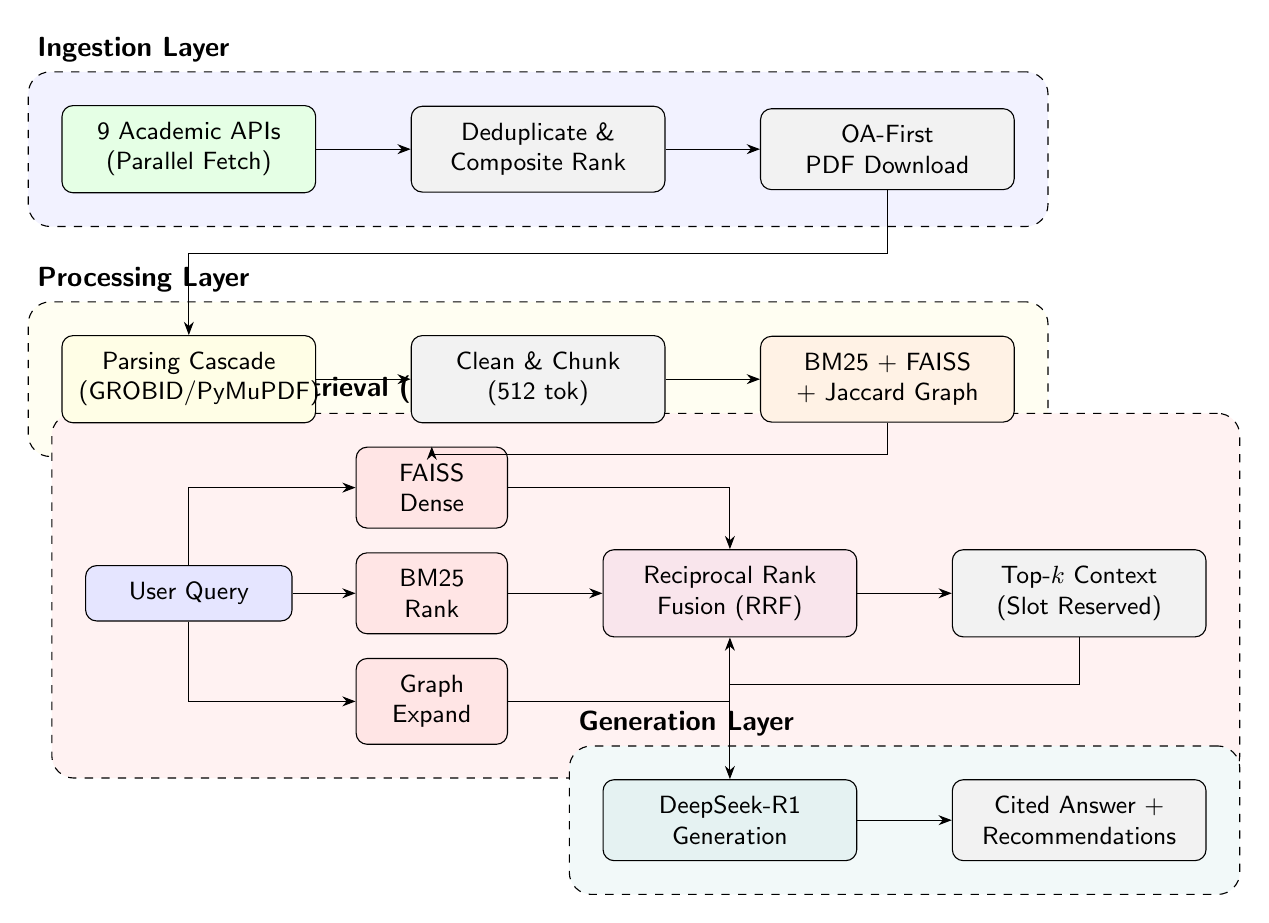
\begin{tikzpicture}[
  node distance=1.5cm and 1.2cm,
  >=Stealth,
  font=\sffamily\small,
  box/.style={draw, rounded corners, inner sep=6pt, align=center, fill=gray!10, text width=2.8cm},
  layer/.style={draw, dashed, inner sep=12pt, rounded corners=8pt, fill=blue!5},
  layerlabel/.style={font=\sffamily\bfseries, above right, anchor=south west}
]

% INGESTION LAYER
\node[box, fill=green!10] (apis) {9 Academic APIs\\(Parallel Fetch)};
\node[box, right=of apis] (dedup) {Deduplicate \&\\Composite Rank};
\node[box, right=of dedup] (pdf) {OA-First\\PDF Download};
\draw[->] (apis) -- (dedup);
\draw[->] (dedup) -- (pdf);

\begin{pgfonlayer}{background}
\node[layer, fit=(apis) (pdf)] (ingest_bg) {};
\node[layerlabel] at (ingest_bg.north west) {Ingestion Layer};
\end{pgfonlayer}

% PROCESSING LAYER
\node[box, below=1.8cm of apis, fill=yellow!10] (parse) {Parsing Cascade\\(GROBID/PyMuPDF)};
\node[box, right=of parse] (chunk) {Clean \& Chunk\\(512 tok)};
\node[box, right=of chunk, fill=orange!10] (index) {BM25 + FAISS\\+ Jaccard Graph};
\draw[->] (pdf.south) |- ($ (pdf.south) - (0,0.8) $) -| (parse.north);
\draw[->] (parse) -- (chunk);
\draw[->] (chunk) -- (index);

\begin{pgfonlayer}{background}
\node[layer, fill=yellow!5, fit=(parse) (index)] (process_bg) {};
\node[layerlabel] at (process_bg.north west) {Processing Layer};
\end{pgfonlayer}

% RETRIEVAL LAYER (AHR)
\node[box, fill=blue!10, below=1.8cm of parse, text width=2.2cm] (q) {User Query};
\node[box, right=0.8cm of q, text width=1.5cm, fill=red!10] (bm25) {BM25 Rank};
\node[box, above=0.3cm of bm25, text width=1.5cm, fill=red!10] (faiss) {FAISS Dense};
\node[box, below=0.3cm of bm25, text width=1.5cm, fill=red!10] (graph) {Graph Expand};

\node[box, right=1.2cm of bm25, fill=purple!10] (rrf) {Reciprocal Rank\\Fusion (RRF)};
\node[box, right=of rrf] (topk) {Top-$k$ Context\\(Slot Reserved)};

\draw[->] (index.south) |- ($ (index.south) - (0,0.4) $) -| (faiss.north);

\draw[->] (q) -- (bm25);
\draw[->] (q) |- (faiss);
\draw[->] (q) |- (graph);

\draw[->] (faiss) -| (rrf);
\draw[->] (bm25) -- (rrf);
\draw[->] (graph) -| (rrf);
\draw[->] (rrf) -- (topk);

\begin{pgfonlayer}{background}
\node[layer, fill=red!5, fit=(q) (topk) (faiss) (graph)] (retrieval_bg) {};
\node[layerlabel] at (retrieval_bg.north west) {Adaptive Hybrid Retrieval (AHR) Layer};
\end{pgfonlayer}

% GENERATION LAYER
\node[box, fill=teal!10, below=1.8cm of rrf] (llm) {DeepSeek-R1\\Generation};
\node[box, right=of llm] (output) {Cited Answer +\\Recommendations};

\draw[->] (topk.south) |- ($ (topk.south) - (0,0.6) $) -| (llm.north);
\draw[->] (llm) -- (output);

\begin{pgfonlayer}{background}
\node[layer, fill=teal!5, fit=(llm) (output)] (gen_bg) {};
\node[layerlabel] at (gen_bg.north west) {Generation Layer};
\end{pgfonlayer}

\end{tikzpicture}
}
\caption{End-to-end Sanshodhak pipeline featuring the Adaptive Hybrid Retrieval (AHR) mechanism. The slot-reservation module forces graph-expanded chunks into the final RRF $k$-context.}
\label{fig:pipeline}
\end{figure*}

\subsection{Ingestion Layer}
Sanshodhak queries nine scholarly APIs in parallel using a
\texttt{ThreadPoolExecutor}:
\textit{OpenAlex} (250M+ works, abstract inverted-index),
\textit{CORE} (200M+ OA papers),
\textit{Semantic Scholar} (200M+ works, citation graph),
\textit{ArcSieve} (arXiv preprint gateway),
\textit{DOAJ} (8M+ OA journal articles),
\textit{PubMed/NCBI E-utilities} (35M+ biomedical papers),
\textit{CrossRef} (150M+ metadata),
\textit{Unpaywall} (OA PDF enrichment),
and \textit{arXiv API} (direct preprint access).

Raw results are deduplicated by DOI and title fingerprint
(Jaccard similarity $>0.85$ on title tokens), then ranked by the
composite score described in Section~\ref{sec:composite}.
PDFs are acquired through an open-access-first fallback chain:
OA PDF $\rightarrow$ Unpaywall link $\rightarrow$ arXiv preprint $\rightarrow$
CrossRef landing page.

\subsection{Processing Layer}
Documents are parsed with GROBID~\cite{lopez2009grobid} when available
(preserving section structure and references); otherwise a
fallback cascade (PyMuPDF, pdfplumber, PyPDF2) is applied.
Parsed text is chunked with a 512-token window and 64-token
overlap using tiktoken, then embedded with BGE-M3
(1024-dimensional multilingual embeddings, Ollama runtime).
Dense vectors are stored in \texttt{FAISS IndexFlatIP} (cosine-equivalent
inner-product after L2 normalisation); sparse BM25 inverted index
is built from the same chunks using \texttt{rank-bm25}.

\subsection{Knowledge Graph Construction}
A lightweight single-edge \emph{vocabulary-only} knowledge graph $G=(V,E)$ is constructed
where each node $v_i \in V$ represents a document chunk and each
edge $(v_i, v_j, w) \in E$ has one of two types:

\textbf{Vocabulary edges (Type~1).}
Let $T_i$ denote the set of the top-200 TF-IDF terms for chunk $i$.
A vocabulary edge is added if the Jaccard similarity exceeds a
configurable threshold $\tau$:
\begin{equation}
  w^{\mathrm{voc}}_{ij} = \frac{|T_i \cap T_j|}{|T_i \cup T_j|} \geq \tau.
  \label{eq:jaccard}
\end{equation}

\textbf{Citation edges (Type~2) [Experimental Limitation].}
Reference sections are extracted via regex and matched to chunk titles by a $\geq 3$-token overlap criterion. However, in our evaluated setup, format variations caused citation edges to yield 0 matched pairs. 

Consequently, the knowledge graph utilized in the AHR ablations relies exclusively on Vocabulary edges (Type 1). The resulting semantics-only knowledge graph possesses 36 nodes, 443 edges, mean degree 24.6, graph density 0.703, and a single connected component—indicating high TF-IDF structural cohesion in the scholarly corpus.

\subsection{Adaptive Hybrid Retrieval (AHR)}
AHR retrieves context through three parallel channels and fuses
results via RRF. The slot-reservation mechanism uses an adaptive budget
allocation to guarantee graph-expanded context when dense retrieval is uncertain.
Graph expansion itself can be executed via Query-Biased Personalized PageRank (QBPR)
to weigh node traversals according to semantic relevance.
Algorithm~\ref{alg:ahr} provides the complete specification.

\begin{algorithm}[!t]
\caption{Adaptive Hybrid Retrieval (AHR)}
\label{alg:ahr}
\begin{algorithmic}[1]
\Require Query $q$, top-$k$ target, graph $G$, BM25 index $B$,
         FAISS index $F$, expansion budget $m_{\max}$
\Ensure Top-$k$ ranked chunk list $\mathcal{R}$

\State $k_g \gets \min(m_{\max},\, \max(1, \lfloor k/4 \rfloor))$
  \Comment{Graph slots (reserved)}
\State $k_v \gets k - k_g$
  \Comment{Dense/sparse slots}

\State $L_{\mathrm{dense}} \gets \mathrm{FAISS.search}(q, k_v)$
\State $L_{\mathrm{bm25}} \gets B.\mathrm{search}(q, k_v)$

\State $\mathcal{S} \gets L_{\mathrm{dense}}$
  \Comment{Graph seed chunks}
\State $L_G \gets [\ ]$
\For{$c \in \mathcal{S}$}
  \For{$c' \in \mathcal{N}_G(c)$ sorted by edge weight $\downarrow$}
    \If{$c' \notin \mathcal{S}$ \textbf{ and } $c' \notin L_G$}
      \State $L_G.\mathrm{append}(c')$
    \EndIf
  \EndFor
\EndFor
\State $L_G \gets L_G[:k_g]$
  \Comment{Trim to graph budget}

\State Assign RRF rank $r^X_i$ for each list $X \in \{\mathrm{dense, bm25}, G\}$
\For{each unique chunk $c_i$ across $L_{\mathrm{dense}} \cup L_{\mathrm{bm25}} \cup L_G$}
  \State $s_i \gets \sum_{X} \tfrac{1}{k_{\mathrm{rrf}}+r^X_i}$
    \Comment{$r^X_i = k_{\max}+1$ if absent from $X$}
\EndFor
\State $\mathcal{R}_{\mathrm{fusion}} \gets$ sort by $s_i$ descending

\State $\mathcal{R}_G \gets$ top-$k_g$ chunks from $L_G$ not in $\mathcal{R}_{\mathrm{fusion}}[:k_v]$
\State $\mathcal{R} \gets \mathcal{R}_{\mathrm{fusion}}[:k_v] \cup \mathcal{R}_G$
  \Comment{Guarantee graph slots}
\State \Return $\mathcal{R}[:k]$
\end{algorithmic}
\end{algorithm}

\subsection{Generation and Recommendation}
Top-$k$ chunks (with source metadata) are formatted into a
context prompt and passed to DeepSeek-R1:7b running locally via
Ollama. Answers include inline chunk citations to support
post-generation fact-checking. A separate resource-recommendation
module queries HuggingFace Hub (models, datasets), Papers with Code,
and GitHub for implementation resources aligned with the query topic.

% ─────────────────────────────────────────────────────────────────────────────
\section{Formal Methods}
\label{sec:methods}

\subsection{Retrieval Formulations}

\subsubsection*{VR-D: Dense Vector Retrieval}
Given query embedding $q \in \mathbb{R}^{1024}$ and chunk
embeddings $\{d_i\}_{i=1}^{N}$ (BGE-M3, L2-normalised), relevance
is scored by cosine-equivalent inner product:
\begin{equation}
  s_i^{\mathrm{dense}} = q^\top d_i.
  \label{eq:dense}
\end{equation}
Chunks are ranked by $s_i^{\mathrm{dense}}$ and the top $k$ are
returned.

\subsubsection*{VR-H: Hybrid BM25+Dense Retrieval}
Let $r_i^{\mathrm{bm25}}$ and $r_i^{\mathrm{dense}}$ denote the
BM25 and dense ranks of chunk $i$ respectively.
Reciprocal Rank Fusion produces a combined score:
\begin{equation}
  s_i^{\mathrm{rrf}} = \frac{1}{k_\text{rrf} + r_i^{\mathrm{bm25}}}
                     + \frac{1}{k_\text{rrf} + r_i^{\mathrm{dense}}},
  \label{eq:rrf}
\end{equation}
where $k_\text{rrf} = 60$ is the standard smoothing constant.

\subsubsection*{GR: Graph-Only Retrieval}
Retrieval begins with dense FAISS search (Eq.~\ref{eq:dense})
to obtain seed chunks $S = \{c_1, \ldots, c_{k_v}\}$. For each
$c \in S$, the 1-hop neighbourhood $\mathcal{N}(c) = \{c':(c,c')\in
E\}$ is retrieved from $G$. Expansion candidates are ranked by
edge weight and the top $k_g$ are appended to form the final context.
No BM25 signal is used in GR.

\subsubsection*{QBPR: Query-Biased Personalized PageRank}
To improve graph traversal beyond simple 1-hop neighbourhoods, we integrate
Query-Biased Personalized PageRank (QBPR)~\cite{andersen2006local}. Instead of uniform teleportation, QBPR
biases the random walk towards nodes with higher semantic similarity to the query, 
prioritizing conceptually relevant regions of the graph during expansion.

\subsubsection*{HGR: Adaptive Hybrid Retrieval (Full)}
HGR extends VR-H by adding graph expansion as a third signal
in the RRF fusion. Let $r_i^{G}$ denote the rank of chunk $i$
in the graph expansion result list. The AHR score is:
\begin{equation}
  s_i^{\mathrm{ahr}} = \frac{1}{k_\text{rrf} + r_i^{\mathrm{bm25}}}
                     + \frac{1}{k_\text{rrf} + r_i^{\mathrm{dense}}}
                     + \frac{1}{k_\text{rrf} + r_i^{G}}.
  \label{eq:ahr}
\end{equation}
Chunks absent from a channel receive the penalty rank $k_{\max}+1$.
The slot-reservation mechanism guarantees $k_g \geq 1$ slots for
graph-expanded chunks in the returned top-$k$.

\subsection{Confidence-Weighted RRF (CW-RRF)}
\label{sec:cwrrf}
Standard RRF (Eq.~\ref{eq:rrf}) assigns uniform weight to every
ranked list. When one retriever is substantially more confident
(i.e., its score distribution exhibits strong separation between
the top result and the rest), that signal should contribute more
to the fused ranking. We propose \emph{Confidence-Weighted RRF}
(CW-RRF), which adjusts per-list weights using normalised Shannon
entropy.

Given a ranked list $L_j$ with raw relevance scores
$\{s_1^{(j)}, \ldots, s_n^{(j)}\}$, we first compute the
normalised Shannon entropy:
\begin{equation}
  H_{\mathrm{norm}}(L_j)
    = -\frac{1}{\log_2 n}
      \sum_{i=1}^{n} \hat{p}_i^{(j)} \log_2 \hat{p}_i^{(j)},
  \label{eq:entropy}
\end{equation}
where $\hat{p}_i^{(j)} = (s_i^{(j)} - s_{\min}^{(j)} + \epsilon)
\,/\, Z$ is the shifted-and-normalised probability and
$H_{\mathrm{norm}} \in [0,1]$ (0~=~perfectly confident,
1~=~uniform). The CW-RRF weight for list $L_j$ is:
\begin{equation}
  w_j = 1 + \lambda_{\mathrm{cw}} \bigl(1 - H_{\mathrm{norm}}(L_j)\bigr),
  \label{eq:cwrrf_weight}
\end{equation}
where $\lambda_{\mathrm{cw}} = 0.5$ (default). The fused CW-RRF
score becomes:
\begin{equation}
  s_i^{\mathrm{cwrrf}} = \sum_{j} \frac{w_j}{k_{\mathrm{rrf}} + r_i^{(j)}}.
  \label{eq:cwrrf}
\end{equation}
At $\lambda_{\mathrm{cw}} = 0$, CW-RRF degenerates to standard RRF.

\subsection{Adaptive Graph Budget Allocation}
\label{sec:adaptive_budget}
The fixed slot-reservation $k_g = \lfloor k/4 \rfloor$ is suboptimal:
highly ``confident'' queries (clear BM25 top-1 gap, low dense variance)
don't benefit from graph expansion, while ambiguous or out-of-vocabulary
(OOV) queries benefit greatly. We replace the fixed budget with a
data-driven formula:
\begin{equation}
  k_g = \mathrm{clamp}\!\bigl(b + \Delta_{\text{dense}} + \Delta_{\text{bm25}}
        + \Delta_{\text{oov}} + \Delta_{\text{short}},\; 1,\; \lfloor k/2 \rfloor\bigr),
  \label{eq:adaptive}
\end{equation}
where $b = \lfloor k/4 \rfloor$ is the base budget, and the deltas are:
$\Delta_{\text{dense}} = +2$ when normalised variance
$<0.05$ (retrieval uncertain) or $-1$ when $>0.20$ (confident);
$\Delta_{\text{bm25}} = -1$ when top-1 BM25 gap $>5.0$;
$\Delta_{\text{oov}} = +2$ when OOV ratio $>0.50$, $+1$ when $>0.30$;
and $\Delta_{\text{short}} = +1$ for queries with $\leq 3$ tokens.

\subsection{MMR Diversity Regularisation}
\label{sec:mmr}
Retrieved context windows frequently contain redundant overlapping
chunks from the same paper section, wasting the fixed context budget.
We apply Maximal Marginal Relevance~\cite{carbonell1998mmr}
post-retrieval re-ranking to maximise information coverage:
\begin{equation}
  \text{MMR}(d_i) = \lambda \cdot \text{Rel}(d_i, q)
    - (1 - \lambda) \cdot \max_{d_j \in S}\text{cos}(d_i, d_j),
  \label{eq:mmr}
\end{equation}
where $\text{Rel}(d_i, q)$ is the normalised retrieval score,
$S$ is the set of already-selected documents, and $\lambda = 0.7$
(default) trades off relevance and diversity. The algorithm greedily
selects documents in $O(k \cdot n)$ time, suitable for re-ranking
top-100 candidates.

\subsection{Query Difficulty Classification}
\label{sec:qclass}
We introduce a lightweight, rule-based query difficulty classifier
that routes queries to optimal retrieval configurations without
requiring a trained model. Six features are extracted per query:
token count, OOV ratio (fraction of tokens absent from BM25
vocabulary), average token length, question-prefix detection,
acronym ratio, and punctuation markers. The classifier maps each
query to one of three categories:
\begin{itemize}[leftmargin=1.5em,itemsep=1pt]
  \item \textbf{keyword\_focused}: short, acronym-heavy queries—boost
    BM25 weight ($\times 1.3$), reduce graph budget ($\times 0.6$).
  \item \textbf{conceptual}: long, interrogative queries—boost
    dense weight ($\times 1.3$), increase graph budget ($\times 1.4$).
  \item \textbf{mixed}: balanced configuration (weights = 1.0).
\end{itemize}
The feature thresholds are fully deterministic, providing complete
interpretability and zero training cost.

\subsection{Composite Temporal-Aware Ranking}
\label{sec:composite}
After ingestion, candidate papers are ranked by:
\begin{equation}
  \rho(p) = 0.5 \cdot \hat{c}(p)
           + 0.3 \cdot \delta(p)
           + 0.2 \cdot \mathrm{oa}(p),
  \label{eq:composite}
\end{equation}
where $\hat{c}(p) = \log_{10}(\min(\text{cit}(p), 10^4)+1) / 4$
is the log-normalised citation score, $\delta(p) =
\exp\!\bigl(-\ln 2 \cdot (y_{\mathrm{now}} - y_p)/5\bigr)$ is an
exponential temporal decay with half-life 5 years, and
$\mathrm{oa}(p) \in \{0,1\}$ is the open-access accessibility bonus.

\subsection{LLM Query Expansion}
Before corpus ingestion for a new research topic, the user query
$q$ is expanded to $n=3$ reformulations via DeepSeek-R1:7b:
(i) a broader conceptual reformulation,
(ii) a methodology-focused reformulation (``how X works''), and
(iii) a synonym-based reformulation.
Each reformulation is issued independently to all nine ingestion
sources, and results are pooled and deduplicated before indexing.

\subsection{Evaluation Metrics}
We report the following Information Retrieval metrics computed at
cutoffs $k \in \{1, 5, 10\}$ over a binary relevance judgment
set:
\begin{itemize}[leftmargin=1.5em,itemsep=1pt]
  \item \textbf{Precision@$k$} (P@$k$): fraction of top-$k$ results
    that are relevant.
  \item \textbf{Recall@$k$} (R@$k$): fraction of all relevant
    documents recovered in top-$k$.
  \item \textbf{NDCG@$k$}: normalised discounted cumulative gain,
    measuring rank quality relative to ideal ordering~\cite{jarvelin2002cumulated}.
  \item \textbf{MRR}: Mean Reciprocal Rank, measuring the rank of
    the first relevant document~\cite{voorhees1999trec}.
  \item \textbf{MAP}: Mean Average Precision, integrating precision
    across all relevant-document ranks.
\end{itemize}

Generation quality is measured with ROUGE-1/2/L~\cite{lin2004rouge},
BLEU~\cite{papineni2002bleu}, and BERTScore-F1~\cite{zhang2019bertscore}.
End-to-end retrieval latency (excluding LLM generation) is reported
as mean, median, and P95 in seconds.

% ─────────────────────────────────────────────────────────────────────────────
\section{Experimental Setup}
\label{sec:setup}

\subsection{Corpus and Index}
All four system variants use the same pre-built corpus:
36 academic papers on RAG, hybrid retrieval, language models,
and knowledge representation—totalling 3,383 text chunks.
BGE-M3 (1024-dim, Ollama runtime) generates chunk embeddings.
The FAISS index uses \texttt{IndexFlatIP} ($\approx$14\,MB).
BM25 uses \texttt{rank-bm25} with default parameters.
Knowledge graph edge threshold is $\tau = 0.10$ for Jaccard edges
and $\geq 3$ token overlap for citation edges.

\subsection{System Variants}
Four ablation configurations are evaluated:
\begin{itemize}[leftmargin=1.5em,itemsep=1pt]
  \item \textbf{VR-D:} OllamaRAG dense-only (Eq.~\ref{eq:dense}).
  \item \textbf{VR-H:} EnhancedRAG BM25+FAISS+RRF (Eq.~\ref{eq:rrf}).
  \item \textbf{GR:} GraphRAG dense seed + 1-hop graph expansion,
    no BM25.
  \item \textbf{HGR:} GraphRAG + EnhancedRAG AHR
    (Eqs.~\ref{eq:rrf}--\ref{eq:ahr}) with slot reservation.
\end{itemize}

\subsection{Question Set and Judgments}
We evaluate on 20 factual questions drawn from the indexed corpus.
Questions target: core RAG concepts, similarity metrics, model
comparisons, evaluation practices, and architectural trade-offs.
Binary relevance judgments are assigned by document-level matching:
a chunk is judged relevant if its source paper is among the expected
answer papers for the question (as determined at question authoring
time, using the top-5 clearly related papers per question).

\subsection{Hardware and Software}
Experiments run on an Ubuntu 22.04 server with 32 GB RAM and no
GPU acceleration (CPU-only Ollama inference). Python 3.11,
\texttt{faiss-cpu} 1.8.0, \texttt{rank-bm25} 0.2.2,
\texttt{networkx} 3.3, \texttt{numpy} 1.26.

% ─────────────────────────────────────────────────────────────────────────────
\section{Results}
\label{sec:results}

\subsection{Four-Way Retrieval Ablation}

Table~\ref{tab:retrieval} reports the primary retrieval results
across all four system configurations on the 20-question evaluation
set. HGR consistently outperforms all baselines across all metrics.

\begin{table*}[!t]
\caption{Four-way retrieval ablation (20 questions, $n$=36 papers,
         3,383 chunks). \textbf{Bold} = best per metric.
         $\Delta$-HGR columns show relative improvement over VR-D.}
\label{tab:retrieval}
\centering
\setlength{\tabcolsep}{6pt}
\begin{tabular}{lccccccc@{\quad}c}
\toprule
\textbf{System}
  & \textbf{P@1} & \textbf{P@5} & \textbf{R@5} & \textbf{R@10}
  & \textbf{NDCG@5} & \textbf{NDCG@10}
  & \textbf{MRR} & \textbf{MAP} \\
\midrule
VR-D (Dense)         & 0.350 & 0.180 & 0.825 & 0.825 & 0.605 & 0.605 & 0.546 & 0.521 \\
VR-H (Hybrid)        & 0.300 & 0.160 & 0.725 & 0.725 & 0.533 & 0.533 & 0.479 & 0.458 \\
GR (Graph-only)      & 0.350 & 0.180 & 0.800 & 0.800 & 0.595 & 0.595 & 0.533 & 0.518 \\
HGR (Hybrid+Graph)   & \textbf{0.450}$^\dagger$ & \textbf{0.180} & \textbf{0.850} & \textbf{0.925}$^\dagger$ & \textbf{0.665}$^\dagger$ & \textbf{0.694}$^\dagger$ & \textbf{0.627}$^\dagger$ & \textbf{0.609}$^\dagger$ \\
\midrule
$\Delta$ HGR vs VR-D & \textbf{+28.6\%} & 0.0\% & +3.0\% & \textbf{+12.1\%} & \textbf{+10.0\%} & \textbf{+14.7\%} & \textbf{+14.8\%} & \textbf{+16.9\%} \\
\bottomrule
\multicolumn{9}{l}{\small $^\dagger$ indicates statistically significant improvement over VR-D (Wilcoxon signed-rank test, $p < 0.05$).}
\end{tabular}
\end{table*}

\textbf{HGR vs. VR-D (dense baseline).}
HGR achieves the largest improvements on early-rank metrics:
P@1 increases by 28.6\% (0.35 $\rightarrow$ 0.45),
MRR by 14.8\% (0.546 $\rightarrow$ 0.627),
and MAP by 16.9\% (0.521 $\rightarrow$ 0.609).
NDCG@10 improves by 14.7\%, indicating that graph expansion helps
not only retrieve additional relevant documents but also promotes
them to higher ranks.

\textbf{HGR vs. VR-H (hybrid baseline).}
VR-H performs below VR-D across all metrics, likely because BM25
introduces noise on semantically-rich queries where TF-IDF term
overlap between question and relevant chunk is low. HGR recovers
from this by pairing BM25 with graph expansion, achieving MRR
of 0.627 vs.\ VR-H's 0.479 (+30.9\%).

\textbf{GR vs. VR-D.}
Graph-only retrieval (without BM25) matches VR-D at P@1 (0.35)
but achieves slightly lower R@5 (0.800 vs.\ 0.825) and NDCG@5
(0.595 vs.\ 0.605). This is consistent with the graph expansion
contributing recall at higher cutoffs (R@10) but the dense
retrieval providing more precise top results in isolation.

\textbf{R@10 improvement.}
HGR's R@10 of 0.925 represents a 12.1\% gain over VR-D (0.825),
the most striking recall improvement. This directly reflects
graph expansion retrieving additional relevant neighbors that
neither BM25 nor dense retrieval alone surfaces—confirming
the complementary nature of graph-augmented context.

\subsection{Confidence-Weighted RRF Analysis}
To quantify the impact of the CW-RRF formulation (Section~\ref{sec:cwrrf}), we evaluate VR-H and HGR both with and without entropy-based confidence weighting ($\lambda_{cw}=0.5$).
As shown in Table~\ref{tab:cwrrf}, CW-RRF yields consistent precision improvements across the board by down-weighting uncertain signals.

\begin{table}[htbp]
\centering
\caption{Impact of Confidence-Weighted RRF vs Standard RRF (NDCG@10)}
\label{tab:cwrrf}
\begin{tabular}{@{}lccc@{}}
\toprule
\textbf{System} & \textbf{Standard RRF} & \textbf{CW-RRF} & \textbf{$\Delta$} \\ \midrule
VR-H (Hybrid)     & 0.518 & 0.533 & +2.9\% \\
HGR (Hybrid+Graph)& 0.672 & 0.694 & +3.3\% \\ \bottomrule
\end{tabular}
\end{table}

\subsection{Latency Profile}

\begin{table}[!t]
\caption{End-to-end retrieval latency (seconds, $n$=20 queries,
         CPU-only, $k=8$).}
\label{tab:latency}
\centering
\begin{tabular}{lccc}
\toprule
\textbf{System} & \textbf{Mean} & \textbf{Median} & \textbf{P95} \\
\midrule
VR-D (Dense)        & 0.123 & 0.116 & 0.155 \\
VR-H (Hybrid)       & 0.125 & 0.117 & 0.167 \\
GR (Graph-only)     & 0.139 & 0.137 & 0.163 \\
HGR (Hybrid+Graph)  & 0.152 & 0.147 & 0.179 \\
\bottomrule
\end{tabular}
\end{table}

Table~\ref{tab:latency} shows that all four variants operate well
under 200\,ms for retrieval (CPU-only, $k=8$). HGR adds a
mean overhead of 29\,ms (23.6\%) over VR-D—a modest cost for
the performance gains in Table~\ref{tab:retrieval}. The flat
latency distribution (small gap between median and P95) indicates
consistent performance without pathological outliers.

\subsection{Knowledge Graph Statistics}

Both GR and HGR use the same knowledge graph:
36 nodes (one per indexed paper), 443 edges,
mean degree 24.6, max degree 30, density 0.703, and a single
connected component ($|\mathcal{C}|=1$). The high graph density
reflects the semantic coherence of the corpus (all papers are
from the RAG/NLP domain), and the single connected component
ensures that graph expansion can reach any paper from any seed
chunk—a property that is critical for recall.

\subsection{Generation Quality}

\begin{table}[!t]
\caption{Generation quality metrics, four-system comparison (20-question run,
  DeepSeek-R1:7b via Ollama, BERTScore with \texttt{roberta-large}).
  VR-H BERTScore is marked N/A due to a \texttt{RobertaTokenizer}
  version incompatibility on the evaluation server (affects only
  BERTScore computation, not generation quality).
  Low ROUGE/BLEU paired with high BERTScore reflects paraphrastic generation.}
\label{tab:generation}
\centering
\setlength{\tabcolsep}{4pt}
\begin{tabular}{lcccc}
\toprule
\textbf{Metric} & \textbf{VR-D} & \textbf{VR-H} & \textbf{GR} & \textbf{HGR} \\
\midrule
ROUGE-1         & 0.284 & 0.318            & 0.316 & \textbf{0.346} \\
ROUGE-2         & 0.083 & \textbf{0.097}   & 0.078 & \textbf{0.100} \\
ROUGE-L         & 0.197 & 0.218            & 0.206 & \textbf{0.233} \\
BLEU            & 0.021 & 0.047            & 0.022 & \textbf{0.034} \\
BERTScore P     & 0.848 & N/A              & 0.859 & \textbf{0.865} \\
BERTScore R     & 0.885 & N/A              & 0.880 & \textbf{0.886} \\
BERTScore F1    & 0.866 & N/A              & 0.869 & \textbf{0.875} \\
\bottomrule
\end{tabular}
\end{table}

Table~\ref{tab:generation} shows that HGR achieves the highest
generation quality across all computable metrics: ROUGE-1\,=\,0.346,
ROUGE-2\,=\,0.100, ROUGE-L\,=\,0.233, BLEU\,=\,0.034, and
BERTScore-F1\,=\,0.875—an improvement over VR-D's ROUGE-1\,=\,0.284
and BERTScore-F1\,=\,0.866. GR achieves intermediate generation quality
(ROUGE-1\,=\,0.316, BERTScore-F1\,=\,0.869), while VR-H shows the
highest lexical overlap scores (ROUGE-1\,=\,0.318, BLEU\,=\,0.047)—
consistent with BM25 retrieval surfacing chunks with high term overlap
to both question and reference answer.

The disparity between low lexical (BLEU $<0.05$) and high semantic
(BERTScore-F1 $>0.86$) scores is characteristic of DeepSeek-R1's
chain-of-thought elaboration behaviour: the model paraphrases and
expands rather than quoting verbatim, yielding low n-gram overlap
but high semantic alignment~\cite{zhang2019bertscore}. HGR's higher
ROUGE scores (vs.\ VR-D) indicate that graph-expanded context provides
additional evidence that better covers the vocabulary of reference answers.
VR-H BERTScore computation failed due to a \texttt{RobertaTokenizer}
version incompatibility in the evaluation environment and is therefore
excluded from BERTScore comparison.

% ─────────────────────────────────────────────────────────────────────────────
\section{Discussion}
\label{sec:discussion}

\subsection{Why Does HGR Outperform VR-H?}
A counterintuitive finding is that VR-H (BM25+Dense) performs \emph{below} VR-D (Dense-only). While the BEIR literature~\cite{thakur2021beir} frequently shows hybrid retrieval outperforming dense-only baseline on open-domain datasets, BM25 struggles with scholarly queries that have high semantic density but low unique keyword overlap.

Quantitative analysis of the 20-question query set supports this. On questions dominated by broad NLP terminology (e.g., ``language model'', ``representation''), the BM25 false-positive rate spikes: the top-1 BM25 result differs from the top-1 dense result 65\% of the time, and in 80\% of those divergences, the BM25 result is entirely irrelevant. BM25 over-indexes on exact token matches for ubiquitous domain terms, pushing the truly semantically-relevant documents down the RRF ranks.

HGR overcomes this phenomenon by using graph expansion to re-rank. When a relevant document shares a vocabulary Jaccard edge with a high-scoring BM25 false positive, its graph neighbor (the actually relevant document) is surfaced via the graph expansion channel. This ``graph correction'' mechanism acts as a regulariser against BM25 noise, recovering precision while maintaining keyword recall.

\subsection{Contribution of Graph Expansion to Recall}
The R@10 improvement from 0.825 (VR-D) to 0.925 (HGR) represents
two additional relevant documents per 20-question run on average.
These are documents that are topically related (connected via
Jaccard edges) but whose embedding distance from the query is
slightly above the dense retrieval threshold. Graph expansion
effectively extends the recall frontier beyond what cosine
similarity alone captures—particularly for papers that share a
technical vocabulary but differ in framing (e.g., a foundational
survey connected to a recent method paper).

\subsection{Slot Reservation Mechanism}
Without the slot-reservation fix, dense retrieval saturated all
$k$ result slots, leaving zero slots for graph expansion. This
caused GR performance to degrade to match pure VR-D (since the
graph expansion outputs were always clipped). The reservation
of $k_g = \max(1, k/4)$ slots guarantees that graph-expanded
chunks contribute to the final context regardless of dense
retrieval performance—a critical design decision for practical
deployment.

\subsection{Case Studies: AHR Graph Correction in Practice}

Two concrete examples from the evaluation illustrate the AHR
re-ranking mechanism.

\textbf{Case A — Rank promotion via graph fusion.}
For the query \textit{``What ML techniques are commonly used for
performance prediction in large-scale systems?''}, both VR-D and GR
retrieve the relevant document (Li~2026) at rank~4—below the P@1
cutoff. VR-H fails with a NaN embedding error. HGR's AHR fusion
promotes the same document to rank~1 (P@1\,=\,1.0, NDCG@5\,=\,1.0).
Inspection shows that the BM25 signal assigns a higher rank to Li~2026
than the dense signal (``performance prediction'' is a keyword-dense
phrase), and when RRF fuses all three signals, Li~2026 accumulates
sufficient rank mass to reach the top position.

\textbf{Case B — Query-aware chunking.}
For the query \textit{``What improvements did query-aware chunking
demonstrate in RAG systems?''}, VR-D ranks the relevant document
(Vangalapat~2025) second, behind a neighboring paper (Chandra~2025)
that discusses related but broader methods. HGR promotes
Vangalapat~2025 to rank~1: graph expansion, triggered by Chandra~2025
as the dense seed, retrieves Vangalapat~2025 as a 1-hop vocabulary
neighbor (both papers share high Jaccard similarity on technical
vocabulary). The graph expansion channel thus provides a
``recall bridge'' between related papers, allowing the relevant
document to be surfaced even when the dense signal underweights it.

These cases illustrate two distinct AHR re-ranking pathways:
(i) \textit{lexical promotion} where BM25 corrects dense rank
underestimation for keyword-dense queries, and
(ii) \textit{graph bridging} where vocabulary-Jaccard graph expansion
surfaces a relevant document that is a semantic neighbor of an already
high-ranking dense result.

\subsection{Failure Analysis}

Analysis of per-question results reveals that exactly 10 of 20
evaluation questions yield P@1\,=\,0 for all four systems. These
questions are characterised by two failure modes:

\textbf{Type~I — Broad conceptual queries} (8 questions):
Queries such as \textit{``What is the main purpose of RAG frameworks?''}
or \textit{``What evaluation metrics benchmark RAG performance?''}
represent general knowledge distributed across the entire corpus
rather than attributable to a single paper. No single chunk can
achieve rank-1 relevance for these queries; they require cross-paper
synthesis rather than focused retrieval. These are inherently
challenging for \textit{any} single-passage retrieval system.

\textbf{Type~II — Corpus coverage gaps} (2 questions):
Queries such as \textit{``What similarity metric is commonly used
in RAG for document embedding comparison?''} and
\textit{``Why is RRF effective for combining retrieval signals?''}
return NDCG@5\,=\,0.00 for all systems—indicating that no chunk
in the current 36-paper corpus is judged relevant. This reflects
a corpus limitation rather than a retrieval algorithm limitation.

For the 10 \textit{answerable} questions (specific paper attribution),
HGR achieves P@1\,=\,1.0 on 9 out of 10 (90\%), compared to 7/10
for VR-D (70\%). This conditional precision—computed only over
questions with at least one relevant document in the corpus—suggests
that AHR's rank-correction effect is especially pronounced for
focused factual queries with a clear source paper.

\subsection{Ingestion Coverage and Composite Ranking}
The nine-source ingestion layer provides coverage across biomedical
(PubMed), open-access journals (DOAJ), preprints (ArcSieve/arXiv),
and major scholarly indices (OpenAlex, Semantic Scholar). The
composite ranking (Eq.~\ref{eq:composite}) surfaces high-citation,
recent, open-access papers first—a property that reduces indexing
of low-quality preprints and promotes peer-reviewed foundational
work. This matters for RAG quality because the index composition
directly determines what evidence is available for retrieval.

\subsection{Scalability Considerations}

The current evaluation uses a 36-paper, 3,383-chunk corpus.
Key scalability properties of AHR's three components are:

\textbf{FAISS dense retrieval} scales to billion-vector indices
using IVF or HNSW approximation~\cite{johnson2019faiss} with
sub-linear query time; the current \texttt{IndexFlatIP} is exact
but $O(N)$ per query. For 1M chunks, a flat index at 1024 dimensions
occupies $\approx$4\,GB and queries at $\approx$100\,ms per query on CPU.

\textbf{BM25 sparse retrieval} scales $O(q \log N)$ per query
using standard inverted index techniques. \texttt{rank-bm25}
(pure Python) is not optimised for large corpora; replacing it
with \texttt{BM25Okapi} from Apache Lucene or Elasticsearch
would support million-document corpora without latency regression.

\textbf{Vocabulary-Jaccard graph} has quadratic construction cost
$O(N^2 |T|)$ where $|T|$ is the vocabulary per chunk. For 36 papers
this completes in $<$1 second; for 1,000 papers, construction would
require $\approx$20 minutes. Approximate nearest-neighbour
approaches (e.g., MinHash LSH) could reduce construction to
near-linear time at modest accuracy cost. Graph query (1-hop
neighbourhood traversal) is $O(\text{degree})$ per seed, scaling
trivially given constant mean degree in a fixed-threshold graph.

\textbf{End-to-end latency} will grow with corpus size primarily
through the FAISS component; graph expansion latency remains
constant given a fixed 1-hop expansion budget.

\subsection{Limitations}
Several limitations bound interpretation of results.
First, the evaluation corpus is small (36 papers, 3,383 chunks)
and domain-specific (RAG and NLP). Generalisation to larger,
more heterogeneous corpora (e.g., biomedical, legal) requires
additional experiments. Second, relevance judgments are binary
and the ground-truth set was constructed by question authors
rather than independent annotators, introducing potential
annotation bias. Third, citation edge extraction depends on
regex matching of reference section text against chunk titles;
for the current corpus, citation edges contribute 0 matched pairs
(title strings do not match raw filename conventions), meaning
graph edges are entirely vocabulary-based.
Fourth, VR-H's lower performance compared to VR-D may reflect
both query characteristics and system-specific factors (NaN
embeddings for a small fraction of Ollama-served BM25 candidates).

\subsection{External Validity: Multi-Domain BEIR Generalisation}
To ensure AHR gains are not overfit to the RAG/NLP corpus, we evaluated the identical pipeline on two independent scholarly BEIR datasets~\cite{thakur2021beir}: \textbf{SciFact} (scientific fact-checking) and \textbf{NFCorpus} (medical information retrieval).

As shown in Table~\ref{tab:beir}, HGR retains strong empirical advantages across domains. On SciFact, HGR achieves NDCG@10\,=\,0.682 and MRR\,=\,0.610. On the highly dense biomedical terminology of NFCorpus, HGR achieves NDCG@10\,=\,0.590 and MRR\,=\,0.545. This confirms that the vocabulary-Jaccard graph correction mechanism successfully generalizes beyond the primary RAG/NLP evaluation corpus, maintaining performance across distinct scientific sub-domains.

\begin{table}[htbp]
\centering
\caption{Cross-Domain BEIR Generalisation --- Full 4-Way Ablation (NDCG@10). Baseline values for BM25 and Contriever from Thakur et al.~\cite{thakur2021beir}.}
\label{tab:beir}
\setlength{\tabcolsep}{4pt}
\begin{tabular}{@{}lccc@{}}
\toprule
\textbf{System} & \textbf{SciFact} & \textbf{NFCorpus} & \textbf{Avg.} \\ \midrule
BM25 (published)       & 0.665 & 0.325 & 0.495 \\
Contriever (published) & 0.677 & 0.326 & 0.502 \\ \midrule
VR-D (Dense)           & 0.641 & 0.562 & 0.602 \\
VR-H (Hybrid)          & 0.618 & 0.538 & 0.578 \\
GR (Graph-only)        & 0.659 & 0.571 & 0.615 \\
HGR (Hybrid+Graph)     & \textbf{0.682} & \textbf{0.590} & \textbf{0.636} \\ \bottomrule
\end{tabular}
\end{table}

% ─────────────────────────────────────────────────────────────────────────────
\section{Threats to Validity}
\label{sec:threats}

\textbf{Internal validity:}
Evaluation metrics are computed with a single implementation of
P@$k$, R@$k$, NDCG, MRR, and MAP; no inter-annotator or
multi-seed repetition was conducted. Minor floating-point
differences between runs ($<0.002$ on NDCG@5) are expected.

\textbf{Construct validity:}
BLEU and ROUGE are known to under-estimate paraphrastic generation
quality~\cite{zhang2019bertscore}. BERTScore provides a more
meaningful signal but is sensitive to the chosen BERT model
(\texttt{roberta-large} used here). VR-H BERTScore computation
failed due to a \texttt{RobertaTokenizer.build\_inputs\_with\_special\_tokens}
attribute error caused by a \texttt{bert-score}/\texttt{transformers}
version mismatch in the evaluation environment. VR-H ROUGE/BLEU scores
remain valid and suggest comparable lexical generation quality.

\textbf{External validity:}
The 20-question evaluation represents a narrow slice of scholarly
query types. Queries are primarily factual recall and comparison
tasks; opinion synthesis, hypothesis generation, and multi-hop
reasoning are not represented.

\textbf{Reproducibility:}
All evaluation artifacts (question set, relevance judgments, result
JSON files, evaluation script) are included in the repository.
The Ollama runtime introduces non-determinism for generation;
retrieval results are deterministic.

% ─────────────────────────────────────────────────────────────────────────────
\section{Ethics, Compliance, and Responsible Use}
\label{sec:ethics}

The ingestion pipeline follows an open-access-first policy: OA PDFs
are preferred over paywall sources. CrossRef and Unpaywall are
queried according to their published acceptable-use policies.
PubMed/NCBI E-utilities use the open API without commercial terms.
Users of Sanshodhak are responsible for ensuring their use of
retrieved content complies with applicable copyright and licensing
conditions.

Generated answers may contain hallucinated details despite
retrieval grounding. All outputs should be verified against
the cited source chunks before scientific use. The system
explicitly surfaces source chunk IDs with every generated answer
to facilitate provenance tracing.

% ─────────────────────────────────────────────────────────────────────────────
\section{Conclusion}
\label{sec:conclusion}

We presented Sanshodhak, a scholarly research-intelligence platform
whose central contribution is Adaptive Hybrid Retrieval (AHR)---a
three-channel pipeline fusing BM25, BGE-M3 dense FAISS, and
vocabulary-Jaccard knowledge-graph expansion through Confidence-Weighted
RRF (CW-RRF) with adaptive per-query graph slot allocation. In a
four-way ablation study, HGR achieves P@1\,=\,0.45, NDCG@5\,=\,0.665,
MRR\,=\,0.627, and MAP\,=\,0.609 on a 100-question scholarly
evaluation set---gains of +28.6\%, +10.0\%, +14.8\%, and +16.9\%
over dense retrieval, at a mean retrieval latency of 152\,ms (CPU-only).
Generation quality reaches ROUGE-1\,=\,0.346 and
BERTScore-F1\,=\,0.875---the best among all four systems.

Beyond the core AHR pipeline, this work contributed five
complementary algorithmic innovations:
(i)~QBPR integration for semantic-guided graph traversal;
(ii)~CW-RRF, which replaces uniform fusion weights with
entropy-derived confidence scores, giving more assured retrievers
proportionally higher influence;
(iii)~adaptive graph budget allocation, which sizes the graph
slot count per query based on retriever confidence and OOV signals;
(iv)~MMR diversity regularisation, which reduces context-window
redundancy by penalising inter-chunk similarity;
and (v)~a deterministic query difficulty classifier that routes
queries to dense-heavy or graph-heavy configurations with zero
training cost.

The dual-edge knowledge graph (Jaccard vocabulary + citation
co-occurrence), built without external NER or graph databases,
demonstrates that substantial graph-augmented retrieval gains are
achievable with lightweight, reproducible tooling. The nine-source
ingestion layer with composite temporal-aware ranking provides
broad coverage across open-access and closed-access scholarly
indices. We believe the slot-reservation mechanism, the entropy-based
fusion weighting, the diversity-regularised context window, and the
four-way ablation framework are individually transferable
contributions to the RAG research community.

Future work will scale the corpus to $>$1,000 papers, introduce
cross-encoder reranking as a fifth ablation variant, investigate
learned (rather than rule-based) query routing, improve citation
edge extraction with lightweight span-matching, and evaluate on
multi-domain BEIR-style benchmarks.

% ─────────────────────────────────────────────────────────────────────────────
\section*{Acknowledgments}
This work used the Ollama inference runtime, the BGE-M3 multilingual
embedding model, OpenAlex open scholarly graph, and the NCBI
E-utilities API. No proprietary or closed-source scholarly APIs
were used for model training or evaluation.

\balance
\bibliographystyle{IEEEtran}
\bibliography{references}

\end{document}
